 % -*- root: ../thesis.tex -*-
\chapter{Uncertainty Quantification for quantum state estimation}
\label{chap:error}

% postivity of quantum states for error regions

















%%%%%%%%%%%%%%%%%%%%%%%%%%%%%%%%%%%%%%%%%%%%%%%%%%%%%%%%%%%%%%%%%%%%%%%%%%%%%%%%
\section{Introduction to Statistics}
\label{sec:error.intro}

The objective of statistical inference is to obtain information about the distribution of a random variable $X$ from observational data.
Here, we focus on the special case of inference in parametric models, which can we described as follows~\cite{Wasserman_2013_All}:
A \emph{parametric model} is a family of distributions $\Prob_{\vec\Theta}$ labeled by a finite number of parameters $\vec\Theta \in \Omega$, where $\Omega \subset \Reals^k$ is called the \emph{state space} of the model.
Then, any function $\estim{\vec\Theta}$ mapping observations to the parameter space $\Reals^k$ is called a \emph{point estimator} for the parameters $\vec\Theta$.
In general, we do not require $\estim{\vec\Theta}$ to map to the state space $\Omega$ as this restriction would preclude many relevant estimators.
However, since we are interested in learning about the distribution $X$, not every estimator is equally useful.
Indeed, the goal should be to find the estimator yielding the parameter value that describes the observed data best.

What we mean by \quotes{best} in this context not only depends on the specific model and what the estimate is supposed to be used for, but also on how we interpret the probabilities.
Broadly speaking, there are two different interpretations of probability, namely the frequentist (or orthodox) interpretation and the Bayesian interpretation~\cite{Hajek_2012_Interpretations,Caves_2000_Probabilities}, which lead to distinct schools of inference~\cite{Kiefer_2012_Introduction,Bolstad_2007_Introduction,Wasserman_2013_All}.
Although the two approaches agree for very simple models or -- under mild regularity assumptions -- in the limit of many measurements, they generally yield different and in some cases even contradictory results~\cite[Sec. 11.9]{Wasserman_2013_All}.

So far we have only discussed point estimators, which yield a single value for the parameters.
However, even if our model describes the data perfectly for some choice of $\vec\Theta$, we cannot exactly recover this value from a finite amount of data due to statistical fluctuations.
The concept of error bars, or more generally error regions, allows for quantifying the uncertainty of a given estimate.
In \cref{sub:intro.frequentist}, we introduce the basic concepts of frequentist inference and the corresponding notion of \emph{confidence regions}.
\Cref{sub:intro.bayesian}, is concerned with Bayesian inference and the corresponding notion of error regions, namely \emph{credible regions}.

% uncertatiny quantification, problem with point estimators

\subsection{Frequentist Statistics}
\label{sub:intro.frequentist}

In the frequentist (or orthodox) framework, the probability of an outcome of a random experiment is defined in terms of its relative frequency of occurrence when the number of repetitions goes to infinity~\cite{Keynes_2007_Treatise,Kiefer_2012_Introduction}.
More precisely, denote the number of repetitions of an experiment by $T$ and the number of times the event under consideration $x$ occurred by $n_T$.
Then, a Frequentist interprets the probability $\Prob(x)$ as the statement that if $T \to \infty$, $\frac{n_T}{T} \to \Prob(x)$.

% probabliities = hypothetical frequencies, not repeatable
For the task of parameter estimation, we assume that the observed data are generated from the parametric model with \quotes{true} parameter $\Theta \in \Omega$, which is unknown.
From a finite number of observations $X_1, \ldots X_N$, we must construct an estimate for $\Theta$ that is close to the true value in some sense.
The function $\hat\Theta$ that maps observations to such an estimate is called a point estimator.
The quality of an estimator is measured by its risk function.
A risk function commonly used for continuous parameter spaces is the mean square error
\[
  \label{eq:frequentist.mean_square}
  \mathcal{L}_{\hat\Theta}(\Theta) := \Exp_\Theta \left( \Norm{\Theta - \hat\Theta(X_1, \ldots, X_N)}^2 \right).
\]
\todo{Make loss without expectation}
Note that \cref{eq:frequentist.mean_square} -- and therefore the performance of a given estimator -- still depends on the unknown true value $\Theta$.
Strategies to make statements independent of the true value include
\begin{definition}
  \label{def:frequentist.optimality_conditions}
  \begin{itemize}
    \item $\hat\Theta$ is called a \emph{uniformly best} estimator, if for all other estimators $\hat\Theta'$ and all values of the true parameter $\Theta \in \Omega$
    \[
      \mathcal{L}_{\hat\Theta}(\Theta) \le \mathcal{L}_{\hat\Theta'}(\Theta).
    \]

    \item $\hat\Theta$ is called \emph{minimax}, if for all other estimators $\hat\Theta'$
    \[
      \sup_{\Theta\in\Omega} \mathcal{L}_{\hat\Theta}(\Theta) \le \sup_{\Theta\in\Omega} \mathcal{L}_{\hat\Theta'}(\Theta).
    \]

    \item $\hat\Theta$ is called \emph{best on average} w.r.t.\ a distribution of the true value $\Theta$ if for all other estimators $\hat\Theta'$
    \[
      \Exp_{\Theta} \mathcal{L}_{\hat\Theta}(\Theta) \le  \Exp_{\Theta} \mathcal{L}_{\hat\Theta'}(\Theta).
    \]

    \item $\hat\Theta$ is called \emph{admissible} if there is no other estimator $\hat\Theta'$ such that
    \[
      \forall\Theta \in \Omega\colon \mathcal{L}_{\hat\Theta'}(\Theta) \le \mathcal{L}_{\hat\Theta}(\Theta)
      \quad\mbox{ and }\quad
      \exists\Theta \in \Omega\colon \mathcal{L}_{\hat\Theta'}(\Theta) < \mathcal{L}_{\hat\Theta}(\Theta)
    \]
  \end{itemize}
\end{definition}
\todo{Citation}
\todo{Discussion of different properties, why no expectation value -> no "singular" regions?}
\todo{Choice is arbitrary!}
\todo{How does this connect with definition of probability?}
\todo{Typical estimators? Max likelihood?}
\todo{No statement about single runs!}
\todo{Likelihood ratio CR?}
\todo{Stein's phenomenon}


% examples (also depends on notion of volume), admissability
However, as already mentioned in the introduction, point estimators cannot convey uncertainty in the estimate.
For this purpose we need to introduce a precise notion of \quotes{error bars}, namely \emph{confidence regions}.
A confidence region $\CR \subset \Omega$ with coverage $\alpha \in [0,1]$ is a region estimator -- that is a function that maps observed data to a subset of the parameter space -- such that the true parameter is contained in $\CR$ with probability greater than $\alpha$
\[
  \label{eq:frequentist.coverage}
  \forall \Theta\in\Omega \colon \Prob_\Theta\left( \CR(X_1, \ldots, X_N) \ni \Theta \right) \ge \alpha.
\]

Similar to point estimators, \cref{eq:frequentist.coverage} does not uniquely determine a confidence region construction.
Furthermore, additional constraints are necessary to exclude trivial constructions such as the following:
Take the region estimator, which is always equal to the full parameter space independent of the data $\CR(X_1, \ldots X_N) = \Omega$, then
\[
  \Prob_\Theta\left(  \CR(X_1, \ldots, X_N) \ni \Theta  \right) = 1 \ge \alpha
\]
for all confidence levels $\alpha$.
Although, this construction trivially fulfils the coverage condition~\eqref{eq:frequentist.coverage}, it does not provide useful information on the uncertainty as it does not restrict the parameter space at all.
Therefore, we have to impose a notion of what constitutes a good confidence region.

Clearly, if we have two confidence regions $\CR_1$ and $\CR_2$ with the same confidence level $\alpha$ and $\CR_1 \subset \CR_2$, then $\CR_1$ is more informative.
More generally, smaller regions should be preferred since they convey more confidence in the estimate and exclude more alternatives.
Therefore, measures of size such as (expected) volume or diameter are commonly used as risk functions for region estimators.
This leads to similar definitions as in \cref{def:frequentist.optimality_conditions} for confidence regions with the additional constraint that \cref{eq:frequentist.coverage} has to be fulfilled.

Since it is crucial for the discussion of confidence regions under constraints, let us explicitly state the following the notion of optimality from~\cite[Def. 2.2]{Joshi_1969_Admissibility}.
Note that in contrast to the previous discussion, it uses \quotes{pointwise volume} as a loss function.
\begin{definition}
  \label{def:frequentist.admissible}
  A confidence region $\CR$ for the parameter estimation of $\theta \in \Omega$ is called (weakly) \emph{admissible} if there is no other confidence region $\CR'$ that fulfils
  \begin{enumerate}
    \item(equal or smaller volume) $\Vol(\CR'(\vec x)) \le \Vol(\CR(\vec x))$ for almost all observations $\vec x$.
    \item(same or better coverage) $\Prob(\CR' \owns \theta) \ge \Prob(\CR \owns \theta)$ for all $\theta \in \Omega$
    \item(strictly better) strict inequality holds for one $\theta \in \Omega$ in (ii) or on a set of positive measure in (i).
  \end{enumerate}
\end{definition}
In words, $\CR$ is admissible if there is no other confidence region $\CR'$ that performs at least as good as $\CR$ and strictly better for some non-negligible settings.
The conditions in Def.~\ref{def:frequentist.admissible} are stated only for ``almost all'' $\vec x$, since one can always modify the region estimators on sets of measure zero without changing their statistical performance.
A different approach is to state condition (i) in terms of the expected volume with the average taken over to the data $\vec x$ for a fixed true parameter $\theta$.
This definition of strong admissibility~\cite[Def.~7.1]{Joshi_1969_Admissibility} is closely related to the definition of admissibility for point estimators in \cref{def:frequentist.optimality_conditions}.


\todo{Today: Asymptotic optimal, adaptive, ...}


\subsection{Bayesian Statistics}
\label{sub:intro.bayesian}

% frequentist: parameters fixed, data random; Bayesian: other way
% two different camps of interpretation: subjective and objective -> only differetnt in interpretation, technically the same
% prior -> Bayes' rule -> posterior

Let us now introduce the Bayesian point of view on inference.
In contrast to the Frequentist's framework, where the existence of a single \quotes{true value} for the model parameter is assumed and the observed data is assumed to be random, Bayesian statistics treats the parameter itself as a random variable.
More precisely, in Bayesian statistics probabilities reflect subjective beliefs and allow for consistently updating one's belief according to empirical observations.
In a parameter estimation problem, the \emph{prior distribution} $\Prob(\Theta)$ expresses one's belief about the parameter $\Theta$ before taking any data into account.
Given an observation $X$, the distribution of $\Theta$ is updated according to Bayes' rule~\cite{}
\[
  \label{eq:bayesian.bayes_rule}
  \Prob(\Theta | X) = \frac{\Prob(X | \Theta) \Prob(\Theta)}{\Prob(X)}.
\]
Here, $\Prob(X|\Theta)$ is the \emph{likelihood function} and $\Prob(\Theta | X)$ is the \emph{posterior distribution} -- or short posterior -- of $\Theta$.

Computing the Bayesian update~\eqref{eq:bayesian.bayes_rule} analytically is possible only in a few rare cases:
If for likelihood function the prior and the posterior are in the same family of distributions, the prior is called a \emph{conjugate prior} for the likelihood function.
For example, consider a Gaussian random variable $X \sim \Normal(\theta, \tau^2)$ with known variance $\tau^2$.
If we assume a Gaussian prior $\theta \sim \Normal(\mu, \sigma^2)$, we have~\cite{}
\[
  \theta \vert X=x \sim \Normal (\mu', \sigma'^2)
\]
with
\[
  \mu' = \frac{ \frac{\mu}{\sigma^2} + \frac{x}{\tau^2} }{ \frac{1}{\sigma^2} + \frac{1}{\tau^2} },
  \quad\mbox{and}\quad
  \sigma' = \left( \frac{1}{\sigma^2} + \frac{1}{\tau^2} \right)^{- \tfrac{1}{2}}.
\]
In other words, an update of a Gaussian prior with a Gaussian likelihood function yields a Gaussian posterior distribution.
Although there are other well-known conjugate priors with explicit formulas for the parameter update, in practice the Bayesian update~\eqref{eq:bayesian.bayes_rule} can only be approximated numerically.
Commonly used methods include sampling techniques such as Markov Chain Monte Carlo and Sequential Monte Carlo~\cite{} as well as variational Bayes~\cite{}.\\


Note that the posterior contains all the information on $\Theta$.
To summarize important features of the posterior, we introduce point and region estimators similar to the Frequentist case:
One commonly used estimator is the Bayesian mean estimator (BME) given by
\[
  \hat\Theta_\mathrm{BME}(X) = \int \Theta \, \Prob(\Theta | X) \, \dd\Theta.
\]
A justification for the BME is that it minimizes (under normal circumstances~\cite{Lehmann_1998_Theory}) the expected loss
\[
  \label{eq:bayesian.expected_loss}
  \Exp_\Theta \mathcal{L}(\Theta, \hat\Theta(X)),
\]
provided the loss function $\mathcal{L}$ is a \emph{Bregman divergence}~\cite{Banerjee_2005_On}.
Note that the expectation over $\Theta$ in \cref{eq:bayesian.expected_loss} is taken over the posterior with observation $X$.

Another example of a point estimator is the \emph{maximum a posteriori} (MAP) estimator.
As the name suggests, the MAP estimator is obtained by maximizing the posterior~\eqref{eq:bayesian.bayes_rule}.
Since this does not require the expensive computation of the denominator in \cref{eq:bayesian.bayes_rule} and (at least local minima) of the posterior can be found efficiently via gradient descent, the MAP estimator is often used in high dimensional problem~\cite{Murphy_2012_Machine}.\\


Let us now introduce the concept of error regions in the Bayesian framework.
A \emph{credible region}\footnote{%
  We use the same letter for confidence and credible regions when the meaning is clear from the context.
}
$\CR$ with credibility $\alpha$ is a subset of the parameter space $\Omega$ containing at least mass $\alpha$ of the posterior
\[
  \label{eq:bayesian.credibility}
  \Prob(\Theta \in \CR | X_1, \ldots, X_N) \ge \alpha.
\]
Notice the different notion of randomness compared to \cref{eq:frequentist.coverage}:
Confidence regions are random variables due to their dependence on the data and \cref{eq:frequentist.coverage} demands that the true value is contained in the confidence region with high probability.
Here, \quotes{probability} refers to (possibly hypothetical) repetitions of the experiment -- no statement can be made for a single run of an experiment with given outcomes.
In contrast, the definition of credible regions~\eqref{eq:bayesian.credibility} only refers to probability w.r.t.\ the posterior and, therefore, is well defined even for a single run of the experiment.

In order to single out \quotes{good} credible regions, we need to introduce a notion of optimality.
As argued in \cref{sub:intro.frequentist}, smaller error regions are generally more informative.
Therefore, good credible regions are minimal-volume credible regions (MVCRs) or credible regions with the smallest diameter.
Since the prior and data are  assumed to be fixed, no ambiguity similar to \cref{def:frequentist.optimality_conditions} arises in this setting.
Although in the following we deal with MVCRs w.r.t.\ a geometric notion of volume, some authors have proposed to measure the volume of a region by its prior probability~\cite{Evans_2006_Optimally,Shang_2013_Optimal}.



\todo{Objective vs subjective Bayesian}






d













%%%%%%%%%%%%%%%%%%%%%%%%%%%%%%%%%%%%%%%%%%%%%%%%%%%%%%%%%%%%%%%%%%%%%%%%%%%%%%%%
\section{Introduction to Complexity Theory}
\label{sec:intro.complexity}

\todo{Ballanced sum problem}
\todo{Hardness, completeness}

\begin{problem}\label{prob:ellpos.balanced_sum}
  Given a vector $\vec a \in \mathbb{N}^d$, decide whether there exists a vector $\vec \psi$ with
  \[
    \forall{k}\:\psi_{k}\in\left\{ -1,1\right\} \;\textrm{ and }\quad \vec a \cdot \vec\psi=0.
    \label{eq:ellpos.partition_vector}
  \]
\end{problem}
In case there is such a vector $\vec \psi$ one says that the instance $\vec a$ allows for a balanced sum partition because the sum of components of $\vec a$ labeled by $\psi_i = 1$ is equal to the sum of components $a_i$ labeled by $\psi_i = -1$.




















%%%%%%%%%%%%%%%%%%%%%%%%%%%%%%%%%%%%%%%%%%%%%%%%%%%%%%%%%%%%%%%%%%%%%%%%%%%%%%%%
\section{Frequentist Confidence Regions}
\label{sec:error.frequentist}

In this section we are going to present the first major result of our work~\cite{Suess_2016_Error} concerned with Frequentist confidence regions in QSE.
Optimal confidence regions for high-dimensional parameter estimation problems in are quite intricate in general even without additional constraints.
There are only few elementary settings, where optimal error regions are known and easily characterized.

Since the goal of this work is to demonstrate that quantum shape constraints severely complicate even ``classically'' simple confidence regions, in the further discussion we restrict the discussion to a simplified setting:
We focus on confidence ellipsoids for Gaussian distributions, which are one of the few easily characterizable examples.
% FIXME REALLY?
As discussed in \cref{sub:intro.frequentist}, Gaussian distributions arise in the limit of many measurements due to local asymptotic normality.
In this section we show that even characterizing these highly simplifying ellipsoids with the quantum constraints taken into account constitutes a hard computational problem.
This simplification is motivated by the goal to show that the computational intractability exclusively stems from the quantum constraints and that it is not caused by difficulties of high-dimensional statistics in general.
Furthermore, any less restrictive formulation encompassing this simplified setting must be at least as hard to solve.

In conclusion, although exploiting the physical constraints may help to reduce the uncertainty tremendously as shown in \cref{FIXME}, doing so in an optimal way is computationally intractable in general.
Therefore, our work can be interpreted as a trade-off between computational efficiency and statistical optimality in QSE.

%%%%%%%%%%%%%%%%%%%%%%%%%%%%%%
\subsection{Optimal confidence regions for quantum states}
\label{sub:ortho.optimal}

% FIXME
As already indicated in \cref{FIXME}, the additional information that the true quantum state $\varrho_0$ must belong to the set of positive semi-definite matrices $\States \subset \HermTrace$ can be exploited to possibly improve any confidence region for QSE.
This is especially clear for notions of optimality with a loss function stated in terms of volume $\Vol(\cdot)$, as we will show in this section.
\todo{Which definition of volume? Should be independent. Maybe proof that truncated voluem can't be double exponentially small?}
We consider an especially simple procedure to take the positivity constraints into account, namely truncating all non-positive matrices from tractable confidence regions for the unconstrained problem.

Although such an ad-hoc approach does not seem to exploit the constraints in an optimal way, it has multiple advantages as we discuss in more detail in \cref{sub:ortho.hard}:
First and foremost, some notions of optimality, e.g.\ admissibility, are preserved under truncation as shown in \cref{lem:ortho.admissible_truncation}.
In other words, there are notions of optimality such that truncation of an optimal confidence region for the unconstrained problem gives rise to an optimal region for the constrained one.
Furthermore, as already mentioned in the introduction, our goal is to show that the intractability arises purely due to the quantum constraints.
Therefore, we start from a tractable solution in the unconstrained setting and show that even this simple approach of taking the constraints into account leads to an computationally intractable problem.
Finally, the truncation approach simplifies the discussion but as we discuss in \cref{sub:ortho.hard}, our results apply to a much larger class of confidence regions such as likelihood ratio based Gaussian ellipsoids.\\


We start by showing that the truncation of confidence regions preservers admissibility.
Notice that \cref{def:frequentist.admissible} can be stated for both, the unconstrained estimation problem $\rho_0 \in \HermTrace$ as well as the constrained estimation problem $\rho_0 \in \States$.
The question is: How are admissible confidence regions for the constrained setting $\CR^+\subset\States$ related to admissible confidence regions for the unconstrained estimation problem $\CR\subset\HermTrace$?
\begin{lemma}\label{lem:ortho.admissible_truncation}
  Let $\CR$ denote an admissible confidence region for the unconstrained estimation problem for the parameter $\varrho_0 \in \HermTrace$.
  Then, the truncated region estimator $\CR^\cap := \CR\cap\States$ is an admissible confidence region for the constrained problem with $\varrho_0 \in \States$.
\end{lemma}
\begin{proof}
  Under the assumption that $\CR^\cap$ is not admissible, there must exist a better confidence region $\CR^+$ for the constrained parameter estimation problem.
  W.l.o.g.\ assume that both $\CR^+$ and $\CR^\cap$ have the same coverage.
  Therefore, we must have $\Vol(\CR^+(\vec y)) \leq \Vol(\CR^\cap(\vec y))$ for almost all observations $y \in \Reals^m$, and there is a set $Y \subset \Reals^m$ of non-zero measure such that $\Vol(\CR^+(\vec y)) < \Vol(\CR^\cap(\vec y))$ for $\vec y \in Y$.
  Define a new confidence region for the unconstrained problem
  \[
    \CR' := \CR^+ \cup \CR^c,
    \label{eq:ortho.new_region}
  \]
  where $\CR^{c}=\CR\setminus \CR^{\cap}$ denotes the compliment of $\CR^{\cap}$ in $\CR$.
  Then, $\CR'$ has the given coverage level, since $\CR^+$ provides coverage for $\varrho_0 \in \States$, whereas $\CR^c$ provides coverage for the case $\varrho_0 \in \HermTrace \setminus \States$.
  Furthermore, we have for almost all $\vec y$
  \[
    \label{eq:ortho.volumes}
    \begin{split}
      \Vol(\CR'(\vec y))
      &= \Vol(\CR^+(\vec y)) + \Vol(\CR^c(\vec y)) \\
      &\leq \Vol(\CR^\cap(\vec y)) + \Vol(\CR^c(\vec y)) \\
      &= \Vol(\CR(\vec y)).
    \end{split}
  \]
  Finally, strict inequality holds in Eq.~\eqref{eq:ortho.volumes} for all $\vec y \in Y$ due to the assumption on $\CR^+$.
  However, this would imply $\CR$ not being admissible in contradiction to the assumptions of the Lemma.
\end{proof}
A similar procedure of computing optimal estimators for constrained problems by modifying an optimal estimator estimator for the unconstrained problem was introduced for the maximum likelihood estimator in~\cite{Smolin_2012_Maximum}.\\



One criticism raised against the use of the truncated confidence regions is the possibility that they may yield empty realizations and, hence, are considered \quotes{unphysical}~\cite{Feldman_1998_Unified}.
However, according to the standard definition in \cref{sub:intro.frequentist}, a procedure that reports 95\% confidence regions is allowed to give any result 5\% of the time.

Furthermore, a different strategy often adopted for point estimator is to use an unconstrained parametrization for the constrained parameter space.
A typical example is a coin toss model with bias $p \in [0, 1]$.
Instead of $p$, the problem can also be parametrized in terms of of log-odds $\log\frac{p}{1 - p}$, which can take any value in $(-\infty,\infty)$.
Similar, one could use the following parametrization for quantum states guaranteed to give a positive semidefinite, Hermitian matrix with trace 1
\[
  \rho(X) = \frac{X \adj X}{\tr X \adj X}
\]
with $X \in \mathbb{C}^{d \times d}$.
Although this parametrization can certainly be advantageous for point estimation, it is unlikely to be helpful for uncertainty quantification:
While $X$ and $\rho(X)$ carry equivalent information, the size of a region measured in \quotes{$X$-space} is hardly related to the size of a region in the physical state space unless one chooses highly unnatural volume measures.
This is necessarily so, as any map from an unbounded space onto the compact quantum state space must grossly distort the geometry.
So, having obtained a \quotes{small confidence region} in parameter space does not imply that the state has been well-estimated w.r.t.\ any physically relevant metric.

%%%%%%%%%%%%%%%%%%%%%%%%%%%%%%
\subsection{Confidence Regions from Linear Inversion}
\label{sub:ortho.linear_inversion}

%%%%%%%%%%%%%%%%%%%%%%%%%%%%%%
\begin{figure*}
  \centering
  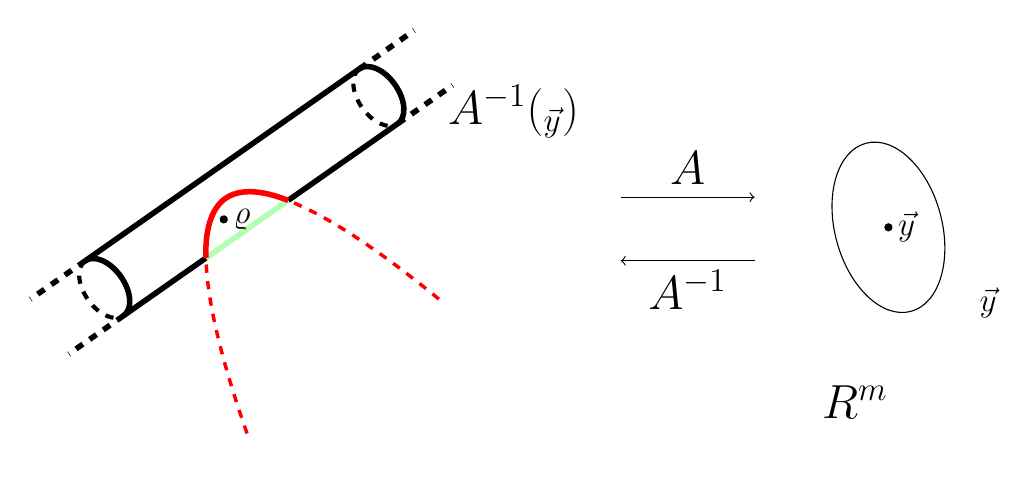
\begin{tikzpicture}[scale=0.85]
    \begin{scope}[shift={(0,0)},rotate=35]
      \draw[line width=2](0,0)--(5,0)  (0,-1)--(1.5,-1)  (3,-1)--(5,-1);
      \draw[dashed, line width=2](0,0)--(-1,0)  (0,-1)--(-1,-1)  (5,0)--(6,0)  (5,-1)--(6,-1);
      \draw[color=green!30!white,line width=2](1.5,-1)--(3,-1);
      \draw[dashed, line width=1.5](0,0) arc (90:270:.3cm and .5cm);
      \draw[dashed, line width=1.5](5,0) arc (90:270:.3cm and .5cm);
      \draw[line width=2](0,0) arc (90:-90:.3cm and .5cm);
      \draw[line width=2](5,0) arc (90:-90:.3cm and .5cm);
      \draw[color=red, line width =2](1.5,-1) parabola bend (2.25,-7/16) (3,-1) ;
      \draw[color=red, dashed, line width =1.25](.5,-3.5) parabola[bend at end] (2.25,-7/16);
      \draw[color=red, dashed, line width =1.25](4,-3.5) parabola[bend at end] (2.25,-7/16);
      \draw[fill=black] (2.05,-.68) circle (1.5pt)  node[anchor=west]{{\large $\estim{{\varrho}}$}};
      \draw[color=red] (1.2,-2.2)  node[anchor=west]{{\LARGE $\States$}};
      \draw (1.2,1.4)  node[anchor=west]{{\LARGE $\HermTrace$}};
      \draw (5.6,-1.2)  node[anchor=west]{{\LARGE $A^{-1}(\CR_{\estim{\vec y}})$}};
    \end{scope}
    \begin{scope}[shift={(7,-2.5)}]
      \draw (0,0) (2,3.5) node[anchor=south]{{\LARGE $A$}} (2,2.5) node[anchor=north]{{\LARGE $A^{-1}$}};
      \draw[->] (1,3.45) -- (3,3.45);
      \draw[<-] (1,2.5) -- (3,2.5);
    \end{scope}
    \begin{scope}[shift={(10,-2.5)}]
      \draw[fill=black] (0,0) (2,3) circle (1.5pt) node[anchor=west]{{\large $\estim{\vec{y}}$}};
      \draw[rotate around={15:(2,3)}] (0,0) (2,3) ellipse (.8 and 1.3);
      \draw (0,0) (3.5,1.5) node[anchor=south]{{\LARGE $\CR_{\estim{\vec y}}$}};
      \draw (0,0) (1.5,0) node[anchor=south]{{\LARGE $\mathbb{R}^m$}};
    \end{scope}
  \end{tikzpicture}
  \caption{\label{fig:ortho.geometry}
    Geometric construction of confidence region for $\estim\varrho$.
    Quantum states are mapped by a measurement matrix $A$ to the respective quantum expectation values $\vec y$.
    Conversely, the pre-image of a confidence region $\CR_{\estim{\vec y}}$ under $A$ gives rise to a confidence region for $\estim\varrho$.
    These may be unbounded if the measurements are not tomographically complete -- a drawback that can be cured by taking into account the physical constraints on quantum states, i.e.\ positivity.
    }
\end{figure*}
\todo{Update figure}
%%%%%%%%%%%%%%%%%%%%%%%%%%%%%%

A particularly simple method to transform estimates of measurement data to estimates of quantum states is the method of \emph{linear inversion}, which we are going to review now:
First, assume that the \emph{true} but unknown quantum state is represented by a $d\times d$ density matrix $\varrho_0$ and QSE performed by measuring $m\geq d^{2} - 1$ tomographically-complete measurement projectors $E_{1},\ldots,E_{m}$.
By $y_{k}=\tr\left(E_{k}\varrho_0\right)$, $k=1,\ldots,m$ we denote the (quantum) expectation values of $E_{k}$ for the true state $\varrho_0$.
Since these relations are linear, we can rewrite them as $\vec{y} = A \vec{\varrho}$, where $\vec{\varrho}$ stands for the quantum state interpreted as a vector and $A$ is the measurement (or design) matrix independent of $\varrho$.
The desired (pseudo)-inverse of the above relation is
\[
  \label{eq:ortho.linear_inversion}
  \vec{\varrho}={\left(A^{T}A\right)}^{-1}A^{T}\vec{y}
\]
and simplifies to $\vec{\varrho}=A^{-1}\vec{y}$ if $m=d^{2} - 1$.

Of course, in an experiment, the expectation values $\vec{y}$ are unknown and can only be approximated by some estimate $\estim{\vec y}$ based on the observed data.
The linear inversion estimate for the quantum state $\estim{\varrho}$ is then given by Eq.~\eqref{eq:ortho.linear_inversion} with the probabilities $\vec y$ replaced by the empirical frequencies $\estim{\vec y}$.
However, due to statistical fluctuations the estimated state $\estim{\varrho}$ is not necessarily positive semidefinite~\cite{Knips_2015_How}, which led to the development of estimators enforcing the physical constraints such as the maximum likelihood estimator~\cite{Hradil_2004_3}.
Although the linear inversion and maximum likelihood estimator solve two distinct problems -- namely the unconstrained and constrained one, respectively -- in certain cases the two are related.
 More precisely, if the outcomes approximately follow a Gaussian distribution, a fast projection algorithm computes the maximum likelihood estimate from the linear inversion estimate directly~\cite{Smolin_2012_Maximum}.

Here, we take a similar approach.
First, the simple geometric interpretation of the linear inversion estimator (see Fig.~\ref{fig:ortho.geometry}) allows us to map confidence regions for the expectation values to confidence regions for the state without taking into account the positivity constraint:
If $\CR_{\estim{\vec y}}$ denotes a confidence region for $\estim{\vec y}$ with confidence level $\alpha$, then so is its pre-image under the measurement map
\[
  \label{eq:ortho.linear_confidence}
  \CR_{\estim{\vec\varrho}} := A^{-1}(\CR_{\estim{\vec y}})
\]
for $\estim{\vec \varrho}$.
Second, the truncation $\CR^\cap_{\estim \varrho} := \CR_{\estim{\vec\varrho}} \cap \States$ yields an improved confidence region for the problem with quantum constraints taken into account.
As shown in Lemma~\ref{lem:ortho.admissible_truncation}, this approach yields admissible confidence region provided the original region was admissible.

The same construction can also be carried out for tomographically incomplete measurements, i.e.\ for $m<d^{2}$:
Since the measurement matrix $A$ is non-invertible in this case, the estimate for the state $\estim{\varrho}$ satisfying $A\estim{\vec\varrho} = \estim{\vec y}$ is not uniquely defined.
However, under additional structural assumptions, one can single out a unique estimate~\cite{Gross_2010_Quantum,Flammia_2012_Quantum}.
The singularity of the measurement map $A$ also reflects in the confidence region defined by Eq.~\eqref{eq:ortho.linear_confidence}.
Even if $\CR_{\estim{\vec y}}$ is a bounded region, the confidence region for the state $\CR_{\estim{\vec \varrho}}$ extends to infinity in the directions \quotes{unobserved by $A$}.
In both cases, the tomographically complete and incomplete, we can use the intersection with the psd states $\States$ to reduce the the region's size while not sacrificing coverage.
This improvement is especially far-reaching in the latter case, where it turns an unbounded region to a bounded one just by taking into account the physical constraints.\\


Of course, the question is whether we can somehow characterize the truncated confidence region $\CR_{\estim{\vec \varrho}}^\cap := A^{-1}(\CR_{\estim{\vec y}}) \cap \States$ computationally efficiently.
Since our goal is to show that this is an intractable problem exclusively due to the quantum constraints -- and not because of the complexity of high-dimensional statistics in general -- we are going to make the simplifying assumption that the measured frequencies are approximately Gaussian distributed.
Furthermore, we are going to focus on a class of confidence regions that are efficiently characterizable in the unconstrained setting, namely Gaussian confidence ellipsoids or, more precisely, ellipsoidal balls of the form
\[
  \CR_{\estim{\vec y}} = \left\{ \vec y \in \Reals^m\colon  {\left(\vec{y}-\estim{\vec{y}}\right)}^T B\left(\vec{y}-\estim{\vec{y}}\right) \leq 1  \right\}
  \label{eq:ortho.confelip}
\]
centered at the the empirical frequencies  $\estim{\vec y}$.
The $m\times m$, symmetric, positive semi-definite matrix $B$ completely specifies the ellipsoidal shape of this confidence region.
These are the natural generalizations of the well-known $2\sigma$ confidence intervals to multivariate Gaussian distributions using likelihood ratios.
\todo{Check the likelihood ratio stuff}

However, even in the unconstrained setting, the ellipsoidal construction~\eqref{eq:ortho.confelip} is known to be admissible only for $m=\left\{ 1,2\right\}$~\cite{Joshi_1969_Admissibility}, while it is not admissible for $m\geq3$~\cite{Joshi_1967_Inadmissibility} due to Stein's phenomenon~\cite{Stein_1956_Inadmissibility}:
By shifting the center of the ellipsoid from the empirical mean $\hat{\vec y}$ to the Stein estimator~\eqref{FIXME}, one can improve the coverage while keeping the volume constant~\cite{Joshi_1967_Inadmissibility}.
Smaller confidence ellipsoids with the same coverage can be obtained by shifting the center slightly~\cite{Tseng_1997_Good,Hwang_1982_Minimax} or use more complicated shapes~\cite{Shinozaki_????_Improved,Brown_1995_Optimal}.
Nevertheless, non of these constructions is known to be optimal and, to the best of the author's knowledge, no optimal confidence region for multivariate Gaussians in dimensions $m \ge 3$ is known.

But since our discussion is focused on the question how the physical psd constraints can be used to improve confidence regions, we are still going to use the ellipsoids~\eqref{eq:ortho.confelip} as a tractable example:
As we will prove later, it is impossible to characterize the truncated ellipsoids efficiently although they are fully described by only few parameters, namely $\estim{\vec y}$ and $B$.\\



In the remainder of this section, we are going to discuss a useful parametrization of the ellipsoids $\CR_{\estim{\vec\varrho}} = A^{-1}(\CR_{\estim{\vec y}})$ with $\CR_{\estim{\vec y}}$ given by \cref{eq:ortho.confelip}.
To this end we use the fact that any $d\times d$ Hermitian matrix can be expanded in a basis formed by the identity $\1$ and $d^{2}-1$ traceless Hermitian matrices $\sigma_{i}$, $i=1,\ldots,d^{2}-1$, normalized according to $\textrm{Tr}(\sigma_{i}\sigma_{j})=2\delta_{ij}$.
With the symbols $\sigma_{i}$ we associate here the most common choice of the basis elements~\cite{Kimura_2003_Bloch}  --  explicitly provided in~\ref{sec:parametrisation} -- while any other $\sigma_{i}'=\sum_{j}O_{ji}\sigma_{j}$, given in terms of an orthogonal $d^{2}-1$ dimensional matrix $O$, are valid alternatives.
For $d=2$ the choice stated in~\ref{sec:parametrisation} is simply the Bloch basis of Pauli matrices: $\sigma_{1}\equiv\sigma_{x}$, $\sigma_{2}\equiv\sigma_{y}$ and $\sigma_{3}\equiv\sigma_{z}$.
In higher dimensions the matrices $\sigma_{i}$ maintain the Bloch basis structure:
Let
\[
  \label{eq:ortho.x_yz_index}
  i_{d}=d(d-1)/2,
\]
then the definition of $\sigma_i$ mimics $\sigma_{x}$ for $1\leq i\leq i_{d}$, $\sigma_{y}$ for $i_{d}+1\leq i\leq2i_{d}$ and $\sigma_{z}$ for $2i_{d}+1\leq i\leq d^{2}-1$.
Therefore, we are going to refer to the $\sigma_{i}$ as \emph{(generalized) Bloch matrices} and the corresponding parametrization of Hermitian matrices as the \emph{(generalized) Bloch representation}.
The following theorem provides a useful parameterization of pre-images under the design matrix $A$ of ellipsoids.
\begin{theorem}\label{thm:ortho.ellipsoids}
  For the tomographically complete case $m \geq d^2 - 1$, the pre-image under the design matrix of any ellipsoid of the form~\eqref{eq:ortho.confelip} can be written as
  \[
    \label{eq:ortho.ellipsoid}
    \CR_{\estim \varrho} = A^{-1}\left( \CR_{\estim{\vec y}} \right) = \left\{ \estim{\varrho} + \sum_{i}R_{i}u_{i}\sigma_{i}'\colon \vec{u}^{T}\vec{u}\leq1 \right\}.
  \]
  Here, $\estim{\varrho}$ is the linear inversion estimator corresponding to \cref{eq:ortho.linear_inversion}, that is a Hermitian matrix with $\tr \estim{\varrho} = 1$. 
  The $R_{i}>0$ ($i=1,\ldots,d^{2}-1$) are the ellipsoid's radii in the directions given by $\sigma_{i}'=\sum_{j}O_{ji}\sigma_{j}$ and the orthogonal matrix $O\in\mathcal{SO}\left(d^{2}-1\right)$ furnishes any orientation of the semi-major axes of the ellipsoid.
\end{theorem}
\begin{proof}
  Note that whenever the sum has no limits specified (like in Eq.~\eqref{eq:ortho.ellipsoid}), by default it extends from $1$ to $d^{2}-1$.
  Let us parameterize both $\varrho \in \CR_{\estim \varrho}$ and $\estim{\varrho}$ in the Bloch representation with coordinates $w_{i}$ and $\estim{w}_i$, respectively:
  \[
    \varrho=\frac{1}{d}\1 + \sum_{i}w_{i}\sigma_{i},
    \qquad\estim{\varrho}=\frac{1}{d} \1 + \sum_{i}\estim{w}_{i}\sigma_{i}.
  \]
  Since $\vec{y}=\textrm{Tr}\left(\vec{E}\varrho\right)$, and $\estim{\vec{y}}=\textrm{Tr}\left(\vec{E}\estim{\varrho}\right)$ we find
  \[
    \vec{y}-\estim{\vec{y}}=Q\left(\vec{w}-\estim{\vec{w}}\right),
  \]
  where $Q$ is a $m\times(d^{2}-1)$ matrix with elements $Q_{ki}=\textrm{Tr}\left(E_{k}\sigma_{i}\right)$.
  In other words, the Bloch coordinates satisfy the same ellipsoid equation (\ref{eq:ortho.confelip}) as the measurement outcomes with $B$ substituted by the $d^{2}-1$ dimensional square matrix $B'=Q^{T}BQ$.
  Since $B$ is symmetric and positive definite, the same holds for $B'$.
  Hence, $B'$ can be diagonalized to the form $B'=ODO^{T}$, where $O \in \mathcal{SO}(d^2 - 1)$ and $D=\textrm{diag}(R_{1}^{-2},\ldots,R_{d^{2}-1}^{-2})$ is the diagonal matrix with positive entries.
  If we rescale $\vec{w}-\estim{\vec{w}}=OD^{-1/2}\vec{u}$, then $\vec{u}^{T}\vec{u}\leq1$ and
  \[
    \varrho-\estim{\varrho}=\sum_{j}\left(\sum_{i}O_{ji}R_{i}u_{i}\right)\sigma_{j}.
  \]
  In the last step of the proof we simply change the orientation of the basis to $\sigma_{i}'=\sum_{j}O_{ji}\sigma_{j}$.
\end{proof}


%%%%%%%%%%%%%%%%%%%%%%%%%%%%%%
\subsection{Computational Intractability of Truncated Ellipsoids}
\label{sub:ortho.hard}

Guided by the discussion from the previous section we now study the confidence region for the linear inversion QST defined as
\[
  \label{eq:ortho.truncated_ellipsoid}
  \CR_{\estim\varrho}^\cap := \CR_{\estim\varrho} \cap \States = A^{-1}(\CR_{\estim y}) \cap \States,
\]
where $\CR_{\estim\varrho}$ is given by the ellipsoid~\eqref{eq:ortho.ellipsoid} for the tomographically complete case $m=d^2 - 1$.
In this section, we are going to show that in contrast to the full ellipsoid $\CR_{\estim\varrho}$, the truncated ellipsoid $\CR_{\estim\varrho}^\cap$ cannot be characterized computationally efficiently.
This shows, for example, in the fact that there is no efficient algorithm to answer the following question:
How much does taking into account the physical constraints reduce the size of the confidence region on a particular set of observed data?
Note that we will not be concerned with properties of the region estimator but with a single instance corresponding to a fixed set of data.
By abuse of notation, we are going to refer to these instances as $\CR_{\estim\varrho}$ and $\CR_{\estim\varrho}^\cap$ as well.

More precisely, we are concerned with the question if a fixed ellipsoid $\CR_{\estim\varrho}$ changes due to the constraints in Eq.~\eqref{eq:ortho.truncated_ellipsoid} or if $\CR_{\estim\varrho}$ is fully contained in the set of psd states.
For the precise formulation, we use the representation of ellipsoids from Thm.~\ref{thm:ortho.ellipsoids}.
\begin{problem}\label{prob:ortho.ellpos}
  Given the center $\estim\varrho$, radii $R_i$, and a basis $\sigma'_i$ for $\HermTrace$.
  Is there a $\vec u \in \Reals^{d^2 - 1}$ with $\vec{u}^{T}\vec{u} \leq 1$ such that
  \[
    \estim{\varrho} + \sum_{i}R_{i}u_{i}\sigma_{i}' \in \HermTrace \setminus \States?
  \]
\end{problem}
The main result of this section is the following statement on the computational complexity of the aforementioned problem.
\begin{theorem}\label{thm:ortho.hard}
  Problem~\ref{prob:ortho.ellpos} is NP-hard.
\end{theorem}
As a consequence of Thm.~\ref{thm:ortho.hard}, the problem of \quotes{characterizing} the truncated confidence ellipsoids $\CR_{\estim{\vec \varrho}}^\cap := A^{-1}(\CR_{\estim{\vec y}}) \cap \States$ defined in Sec.~\ref{sub:ortho.linear_inversion} computationally is hard in general.
By characterizing we mean computing any property of $\CR_{\estim{\vec \varrho}}^\cap$ that is sensitive to whether the truncation influences the original ellipsoid or not, e.g.\ computing the volume of the truncated ellipsoid or its distance to boundary of the quantum state space with high enough precision.
\todo{Proof this! Truncated volume may not become double exponentially small}
Note, however, that there are also properties such as the diameter that might be unaffected by the truncation in certain special cases and, hence, their computational complexity cannot be classified using Thm.~\ref{thm:ortho.hard}.
Furthermore, the more general problem of characterizing truncated confidence regions in general (without the Gaussian approximation) is hard as well since it subsumes Prob.~\ref{prob:ortho.ellpos}.

Another consequence of the theorem concerns confidence regions for the constrained problem, which output ``good regions'' for the unconstrained problem when the constraints are not active:
More precisely, it is extremely natural to use likelihood ratio-based ellipsoidal confidence regions for unconstrained Gaussian data although they cannot be optimal due to Stein's phenomenon.
So it is natural to require any quantum region estimator to behave this way in the particular case that the likelihood function is concentrated well away from the boundary of state space.
What Thm.~\ref{thm:ortho.hard} shows is that any region estimator subject to this criterion must necessarily solve NP-hard problems.\\


Finally, the remainder of this section is dedicated to give some insight to the proof of the main theorem and to discuss a tractable solvable special case.
The proof of Thm.~\ref{thm:ortho.hard} is inspired by a similar result due to Ben-Tal and Nemirovski~\cite{Tal_1998_Robust} in robust optimization theory, who showed that the following problem is NP-complete.
\begin{problem}
  \label{prob:ortho.bental}
  Given $k \in \Naturals$ and $k$ $d\times d$ symmetric matrices $A_{1},\ldots,A_{k}$, check whether there is a $\vec u \in \Reals^k$ with $\vec{u}^{T}\vec{u} \leq 1$ such that $\sum_{i=1}^{k}u_{i}A_{i} > \1_{d}$.
\end{problem}
Although the two problems are strongly related, the intractability result~\cite{Tal_1998_Robust} cannot be applied directly to our QSE related problem due to the following crucial difference:
The proof of NP-hardness of Prob.~\ref{prob:ortho.bental} constructs a reduction of the balanced sum problem~\eqref{FIXME} to the special case of \cref{prob:ortho.bental} with $k=\frac{d(d-1)}{2} + 1$ and real symmetric matrices $A_i$, which are not necessarily pairwise orthogonal to each other~\cite[Sec.~3.4.1]{Tal_1998_Robust}.
However, in Prob.~\ref{prob:ortho.ellpos}, the $\sigma'_i$ ($i=1,\ldots,d^2 - 1)$ form an orthogonal basis of the space of complex Hermitian, traceless matrices.
Hence, we need to adapt the original proof strategy to deal with the restrictions imposed by our QSE related problem.

% Note that the intractability result~\cite{Tal_1998_Robust} does not directly apply the Problem~\ref{prob:ortho.bental}.
% Although our proof uses the same basic idea as the stated result, it had to be adjusted to the geometrical picture of the space of quantum states.
% The wider freedom of the above problem refers to the fact that both parameters $k$ and $l$, together with all $k$ matrices $\left\{ A^{i}\right\} $ are treated as an input.
% In other words, in such a general formulation, it counter-intuitively might be easier to find the hard instances of the problem, as one can freely fix all the degrees of freedom.
% For instance, the desired reduction to an NP-complete problem was shown for $k=l(l-1)/2+1$ and a set of non-orthogonal matrices $(A_k)_k$~\cite[Sec.~3.4.1]{Tal_1998_Robust}.
% Let us emphasize the three main limitations of our tomography-related problem in comparison with the general result cited above:
% \begin{enumerate}
%   \item We deal with complex Hermitian matrices and fixed dimensions $l=d$, $k=d^{2}-1$.
%   \item Our matrices $\left\{ A^{i}\right\}$ are fixed at $\left\{ \sigma_{i}\right\} $, i.e.~they form the generalized Bloch basis of orthogonal matrices.
%   \item The crucial part of the problem by Ben-Tal and Nemirovski can be reformulated as: \emph{do all the matrices $\1_{l}+\sum_{i=1}^{k}u_{i}A^{i}$ belong to $\States$ for $\forall_{u}\vec{u}^{T}\vec{u}\leq1$?} In our case the role of $\1_{l}$ is played by the estimate state $\estim{\varrho}_{0}$
% \end{enumerate}
% The last point above and the problem of deciding whether a confidence ellipsoid is fully contained in the set of psd states are related by Thm.~\ref{thm:ortho.ellipsoids}.
% Therefore, the precise formulation of the latter problem reads
% A negative answer to this problem shows that the corresponding ellipsoid is fully contained within the psd states.


Let us start the outline of the proof of \cref{thm:ortho.hard} with a simplified example: 
Consider $R_{i}=R$ for all $i=1,\ldots,d^{2}-1$ that is all radii are equal and the ellipsoid is a ball.
With no loss of generality, we can assume $\sigma'_i = \sigma_i$.
The following Lemma, which is proven in~\cref{FIXME}, provides an easily checkable, necessary, and sufficient condition to decide \cref{prob:ortho.ellpos} for this special case.
\todo{Remove proof since it's not mine and not crucial?}
\begin{lemma}\label{lem:ortho.spheres}
  Let $\CR$ denote a ball parameterized according to \cref{thm:ortho.ellipsoids} with with radii $R_i=R$ and midpoint $\estim{\varrho}$.
  $\CR$ is fully contained in the set of psd density matrices if and only if
  \[
    R\leq\sqrt{\frac{d}{2\left(d-1\right)}} \, \operatorname{mineig} \estim{\varrho},
  \]
  where $\operatorname{mineig}\estim{\varrho}$ denotes the smallest eigenvalue of $\estim{\varrho}$.
\end{lemma}
The statement is a straightforward but interesting extension of the known result that the largest ball centered at the completely mixed state and fully contained in the set of psd density matrices has radius $R_{\mathrm{max}}=\sqrt{\frac{1}{2d\left(d-1\right)}}$.
Intuitively, when the center of the ball is moved away from the completely mixed state, the allowed radii become smaller.
This correction happens to be quantified by the smallest eigenvalue of the new center.
In conclusions, spherical ellipsoids do not constitute hard instances of \cref{prob:ortho.ellpos} provided that the minimal eigenvalue of $\estim\varrho$ can be computed efficiently with high enough accuracy.

However, it turns out that a slightly more complicated setting is already enough to proof the computational intractability.
The ellipsoids under consideration still have their semi-major axes aligned with the generalized Bloch basis, that is we assume $\sigma'_i = \sigma_i$.
The only change compared to the previous setting is the choice of radii.
We consider the same radius $R_{1}$ for all directions generalizing the $x$-direction to higher dimensions and the distinct radius $R_{2}$ for the remaining directions:
\[
  \label{eq:ortho.subclass}
  \begin{split}
    R_{i}=R_{1} &\quad i=1,\ldots,i_{d}\\
    R_{i}=R_{2} &\quad i=i_{d}+1,\ldots,d^{2}-1.
  \end{split}
\]
Recall the definition of $i_d$ \cref{eq:ortho.x_yz_index}.
To prove the hardness of \cref{prob:ortho.ellpos}, we use a reduction from the balanced sum problem~\ref{prob:ellpos.balanced_sum}.
The main technical difficulty is to identify the values of $R_1$ and $R_2$ as well as $\estim{\rho}$ depending on an instance of the balanced sum problem $\vec a$ such that the corresponding ellipsoid $\CR$ given by \cref{thm:ortho.ellipsoids} contains an element with negative eigenvalues if and only if $\vec a$ has a balanced sum partition.
For the details, please see \cref{sec:ellpos}.















%%%%%%%%%%%%%%%%%%%%%%%%%%%%%%%%%%%%%%%%%%%%%%%%%%%%%%%%%%%%
\section{Bayesian Credibility regions}
\label{sec:bayesian}

\subsection{MVCR for Gaussians}
\label{sub:bayesian.gaussian}

We now turn to the question of minimal volume credible regions (MVCR) in the Bayesian framework:
In the unconstrained case, Gaussian posteriors are one of the few examples of multivariate distributions, where the MVCR are simple geometric objects, namely ellipsoids.
In practice, Gaussian posteriors arise in the following scenario:
Consider a random vector $\vec X\sim\mathcal{N}(\vec\mu, \Sigma)$, where the covariance matrix $\Sigma$ is known and we wish to estimate its mean $\vec\mu$.
If we furthermore assume a Gaussian prior for the mean, the posterior will be Gaussian as well due to the fact that the Gaussian distribution is its own conjugated prior.

This is one of the few cases, in which the Bayesian update as well as the computation of an optimal credible region can be carried out analytically.
First, computing the parameters for the Gaussian posterior distribution can be done by means of \emph{linear Kalman filter update equations}, see e.g.~\cite[Sec.\ 2.4]{Audenaert_2009_Quantum}.
Second, for the credible region, assume that after the Bayesian update, the posterior distribution of $\vec\mu$ is parameterized by its mean $\vec\theta \in \Reals^N$ and covariance matrix $\Sigma \in \Reals^{N \times N}$.
Therefore, the posterior of $\vec\mu$ has probability density
\begin{equation}
  \label{eq:bayesian.gaussian_density}
  \pi_{\vec\theta,\Sigma}(\vec x) = {(2\pi)}^{-\Nhalf} \abs{\Sigma}^{-\frac{1}{2}} \exp\left( -\frac{1}{2} \norm{\vec x - \vec\theta}_\Sigma^2 \right).
\end{equation}
where
\begin{equation}
  \norm{\vec x - \vec\theta}_\Sigma := \sqrt{{(\vec x - \vec\theta)}^T \Sigma^{-1} (\vec x - \vec\theta)}
\end{equation}
is the Mahalanobis distance and  $\abs{\Sigma}$ denotes the determinant of $\Sigma$.
As elaborated in Sec.~\ref{sub:intro.error_regions}, the MVCRs are exactly the highest posterior density sets as defined in Eq.~\eqref{eq:intro.highest_posterior}.
Therefore, the MVCR with credibility $\alpha$ for the density Gaussian~\eqref{eq:bayesian.gaussian_density} is given by
\begin{equation}
  \label{eq:bayesian.gaussian_cr}
  \CR = \{ \vec x \in \Reals^N\colon \norm{\vec x - \vec\theta}_\Sigma \le r_{\alpha} \} =: \Eps(r_{\alpha}).
\end{equation}
This is an ellipsoid centered at $\vec\theta$ with radius $r_{\alpha}$ determined by the saturated credibility condition~\eqref{eq:intro.credible_region}:
\begin{equation}
  \label{eq:bayesian.radius}
  \begin{split}
    \alpha
    &= {(2\pi)}^{-\Nhalf} \abs{\Sigma}^{-\frac{1}{2}} \int_{\Eps(r_{\alpha})} \exp\left( -\frac{1}{2} \norm{\vec x - \vec\theta}_\Sigma^2 \right) \dd^N x \\
    &= \frac{\gamma\left( \Nhalf, \frac{r^2_{\alpha}}{2} \right)}{\Gamma\left( \Nhalf \right)}
    \equiv P\left( \Nhalf, \tfrac{r^2_{\alpha}}{2} \right).
    \end{split}
\end{equation}
By $\gamma(\cdot,\cdot)$ we denote the incomplete $\Gamma$-function and $P(\cdot,\cdot)$ is its normalized version.
The above condition fixes $r_{\alpha}$ uniquely since $x \mapsto P(\Nhalf, x)$ is strictly monotonic for any $N > 0$.
Hence, determining the MVCR for a multivariate Gaussian posterior with known mean and covariances reduces to computing the radius $r_\alpha$, which is formalized in the following problem.
\begin{problem}\label{prob:bayesian.cr}
  For given mean $\vec\theta \in \Reals^N$, covariance matrix $\Sigma \in \Reals^{N \times N}$ with $\Sigma \geq 0$, credibility $\alpha \in [0,1]$, and accuracy $\delta$ with $\delta^{-1} \in \mathbb{N}$, determine the radius of the MVCR $r_{\alpha}$ defined in Eq.~\eqref{eq:bayesian.radius} with given accuracy.
\end{problem}

An efficient algorithm for solving Prob.~\ref{prob:bayesian.cr} is outlined in the following.
To ease notation, we set $x = r^2_{\alpha}/2$.
\begin{enumerate}
  \item W.l.o.g.\ we can assume that $\alpha \le 0.9$ (or some other arbitrary constant).
  Otherwise, the problem can be restated in terms of $Q(\Nhalf, x) = 1 - P(\Nhalf, x)$, which allows for a similar analysis.
  The condition $\alpha \le 0.9$ restricts the search space for $x$ to some finite interval $[0, t_\mathrm{max}]$.
  Note that the upper bound $t_\mathrm{max}$ grows at worst polynomially in $\Nhalf$.
  \item The above restriction, the finite precision, and the fact that $x \mapsto P(\Nhalf, x)$ is strictly monotonic allow for interpreting the problem of finding $x$ given $\alpha$ as a search in an ordered, finite list of size $M \sim \tfrac{t_\mathrm{max}}{\delta}$.
  \item Each entry of this list can be evaluated with exponential precision in polynomial time using a power series expansion of $P(\Nhalf, x)$ (for more details see Lemma~\ref{lem:bayesian.normalization_constant} in~\ref{sec:proof_bayesian}).
  \item Since finding $x$ in this list only requires $\log M$ evaluations using binary search, the whole problem can be solved in polynomial time.
\end{enumerate}


%%%%%%%%%%%%%%%%%%%%%%%%%%%%%%
\subsection{Bayesian QST}
\label{sub:bayesian.tomography}

%%%%%%%%%%%%%%%%%%%%%%%%%%%%%%%%%%%%%%%%%%%%%%%%%%%%%%%%%%%%%%%%%%%%%%%%%%%%%%%
\begin{figure*}[t]
  \centering
  \begin{tikzpicture}[
    elip/.style={fill=yellow, line width=0},
    truncated/.style={pattern=north west lines, pattern color=blue},
    truncelip/.style={dashed, line width=2pt, fill=blue},
    psd/.style={dashed, color=red, line width=2pt}
  ]
    \clip (-3,-3) rectangle (13,3);

    \def\origelip{(0,0) ellipse [x radius=1.5, y radius=2, rotate=-30]}
    \def\truncatedelip{(0,0) ellipse [x radius=2, y radius=2.66666, rotate=-30]}

    \def\psdradius{5.5}
    \def\psdcircle{(psdcenter) [draw=none] circle (\psdradius)}

    \begin{scope}[shift={(0,0)}]
      \draw[elip]\origelip;
      \draw[truncated]\origelip;
      \node at (0.2,0) {$\Eps(r_{\frac{\alpha}{C}})$};
      \node at (2.4,-.2) {$\Eps(r^+_{\alpha})$};


      \node at (0,-3) (psdcenter) {};
      \node[color=red] at (3,1) {psd};
      \draw[psd] ([shift=(50:\psdradius)]psdcenter) arc (50:100:\psdradius);
    \end{scope}


    \begin{scope}[shift={(8,0)}]
      \draw[truncelip]\origelip;
      \draw\truncatedelip;

      \node at (-1,-4) (psdcenter) {};
      \node[color=red] at (3,1) {psd};

      \draw[psd] ([shift=(50:\psdradius)]psdcenter) arc (50:100:\psdradius);
      \begin{scope}
        \clip \psdcircle;
        \fill[elip] \origelip;
        \fill[truncated]\truncatedelip;
      \end{scope}

      \node at (0,0) {$\Eps(r_{\frac{\alpha}{C}})$};
      \node at (2.8,-.4) {$\Eps(r^+_{\alpha})$};
    \end{scope}
  \end{tikzpicture}
  \caption{\label{fig:bayesian.ellipsoids}
    The two possible cases for the credible regions.
    \emph{Left:} The original ellipsoid $\Eps(r_\frac{\alpha}{C})$ with credibility $\frac{\alpha}{C}$ (yellow) lies completely inside the psd states and is, therefore, equal to the ellipsoid taking into account positivity $\Eps(r^+_{\alpha})$ with credibility $\alpha$ (blue hatched).
    \emph{Right:}  Parts of the original ellipsoid $\Eps(r_\frac{\alpha}{C})$ lie outside the psd states (blue).
    Hence, the ellipsoid that takes into account positivity $\Eps(r^+_{\alpha})$ has to have a larger radius in order to achieve the sought for credibility.
  }
\end{figure*}
%%%%%%%%%%%%%%%%%%%%%%%%%%%%%%%%%%%%%%%%%%%%%%%%%%%%%%%%%%%%%%%%%%%%%%%%%%%%%%%

Let us now turn to the application of Bayesian methods to QST, for a more thorough discussion see e.g.~\cite{Granade_2015_Practical}.
%Here, the parameter we want to estimate is a quantum state
%\begin{equation}
 % \varrho \in \States = \{ \varrho \in \BC^{d \times d}\colon \varrho = \varrho^\dagger, \tr \varrho = 1, \varrho \ge 0 \}.
%\end{equation}
%Here, $\States$ denotes the set of valid mixed quantum states, which is a proper subset of the real vector space $\HermTrace$ of hermitian matrices with trace 1.
In order to incorporate the prior knowledge of positive semidefiniteness, we chose a prior that is concentrated on $\States$ and vanishes on its complement.
As before% in Sec.~\ref{sub:bayesian.gaussian}
, we choose a (truncated) Gaussian prior and, therefore, Gaussian posteriors.
Hence, the density $\pi_{\theta,\Sigma}^+(\varrho)$ of a Gaussian posterior on $\States$ with respect to the flat Hilbert-Schmidt measure $\dd\varrho$ on $\HermTrace$ can be written as
\begin{equation}
  \label{eq:bayesian.density_plus}
  \pi^+_{\theta,\Sigma}(\varrho) = C_{\theta,\Sigma}\ \chi(\varrho)\ \pi_{\theta,\Sigma}(\varrho).
\end{equation}
Here, $\pi_{\theta,\Sigma}$ is the multivariate Gaussian from Eq.~\eqref{eq:bayesian.gaussian_density} with $\theta \in \HermTrace$.
The other factors in Eq.~\eqref{eq:bayesian.density_plus} ensure that $\pi^+_{\theta,\Sigma}$ is a proper probability distribution supported on $\States$:
$\chi(\varrho)$ is the indicator function of $\States$ and $C_{\theta,\Sigma}$ is the normalization constant defined by
\begin{equation}
  C_{\theta,\Sigma}^{-1} = \int_{\States} \pi_{\theta,\Sigma}(\varrho) \,\dd\varrho.
\end{equation}
From now on we will drop the subscripts indicating the mean $\theta$ and the covariance matrix $\Sigma$ if no confusion arises. It is then important to remember that the constant in question is denoted by $C$, while the credibility region is $\CR$.

The problem we try to solve is the following:
Given the mean $\theta$, covariance matrix $\Sigma$, and credibility $\alpha$, can we find the MVCR for the Gaussian distribution supported on $\States$?
Since the posterior density~\eqref{eq:bayesian.density_plus} is supported on the psd states and MVCRs are highest-density sets due to~\eqref{eq:intro.highest_posterior}, the MVCR is of the form
\begin{equation}
  \Eps(r^+_{\alpha}) \cap \States = \{ \varrho \in \States \colon \norm{\varrho - \theta}_\Sigma \le r^+_{\alpha} \}.
  \label{eq:bayesian.mvcr}
\end{equation}
Similar to Eq.~\eqref{eq:bayesian.radius}, the radius is determined by the credibility condition
\begin{equation}
  \label{eq:bayesian.radius_plus}
  \alpha = C \int_{\Eps(r^+_{\alpha}) \cap \States} \pi_{\theta,\Sigma}(\varrho) \dd \varrho.
\end{equation}
However, this case involves the normalization constant $C$ from~\eqref{eq:bayesian.density_plus} and the integral is restricted to the psd states.
Also, there is no closed-form analogue to Eq.~\eqref{eq:bayesian.radius} due to the psd constraint.

%%%%%%%%%%%%%%%%%%%%%%%%%%%%%%
\subsection{Computational Intractability}
\label{sub:bayesian.hard}






Our main result from this section concerns MVCR for Gaussian posteriors that are fully supported on the psd states.
We will show that the following problem is computational hard.
\begin{problem}\label{prob:bayesian.trucated_cr}
  For given mean $\theta \in \HermTrace$, covariance matrix $\Sigma$, credibility $\alpha \in [0,1]$, and accuracy $\delta$ with $\delta^{-1} \in \mathbb{N}$, determine the radius of the MVCR $r^+_{\alpha}$ defined in Eq.~\eqref{eq:bayesian.radius_plus} with given accuracy.
\end{problem}
In other words, there is no efficient algorithm that outputs smallest volume credibility regions for every Gaussian distribution on $\HermTrace$ restricted to the positive semidefinite states and every credibility $\alpha$.
Consequently, there cannot be an efficient algorithm to solve the problem of MVCR for QST, since the latter more general problem contains the instances of Prob.~\ref{prob:bayesian.trucated_cr}.
To prove Prob.~\ref{prob:bayesian.trucated_cr}, we use a reduction from Problem~\ref{prob:ortho.ellpos}, which has already been shown to be NP-hard.
This reduction runs along the following lines:
\begin{enumerate}
  \item Assume that Prob.~\ref{prob:bayesian.trucated_cr} can be solved efficiently.

  \item As we will prove later, every ellipsoid $\Eps^*$ in $\HermTrace$ can be encoded as a minimum volume credible ellipsoid for some Gaussian distribution $\pi$ with a suitable choice of $\theta$, $\Sigma$, and $R$:
  \begin{equation}
    \Eps^* = \Eps_{\theta,\Sigma}(R).
  \end{equation}
  Note that only $\theta$ is uniquely defined.
  $\Sigma$ is defined only up to a multiplicative, positive constant, since every rescaling of $\Sigma$ can be compensated by an appropriate rescaling of $R$.

  \item  Using the assumed efficient algorithm for Prob.~\ref{prob:bayesian.trucated_cr}, we can compute the normalization constant $C$ of the truncated distribution~\eqref{eq:bayesian.density_plus} for given $\theta$ and $\Sigma$ with sufficient precision in polynomial time.

  \item Based on this, we can compute a credibility $\alpha$ such that $R = r_\frac{\alpha}{C}$ and, therefore,
  \begin{equation}
    \Eps^* = \Eps_{\theta,\Sigma}(r_\frac{\alpha}{C}).
  \end{equation}

  \item The crucial observation is that this ellipsoid is contained in the psd states if and only if the corresponding MVCR for the truncated distribution $\pi^+$ fulfills
  \begin{equation}
    \label{eq:bayesian.criterion}
    r^+_{\alpha} = r_\frac{\alpha}{C}.
  \end{equation}
  See Fig.~\ref{fig:bayesian.ellipsoids} for an illustration.
  Since we can compute $r^+_{\alpha}$ efficiently by assumption, checking Eq.~\eqref{eq:bayesian.criterion} allows us to decide Prob.~\ref{prob:ortho.ellpos}.
\end{enumerate}

In conclusion, the main result from this section is the following lower bound on the computational complexity of Problem~\ref{prob:bayesian.cr}.
\begin{theorem}\label{thm:bayesian.hardness}
  If Problem~\ref{prob:bayesian.trucated_cr} has a polynomial time algorithm, then we can also decide Problem~\ref{prob:ortho.ellpos} in polynomial time.
  Therefore, there is no efficient algorithm for Problem~\ref{prob:bayesian.trucated_cr} unless $\mathrm{P} = \mathrm{NP}$.
\end{theorem}

The proof runs along the lines outlined above and can be found in~\ref{sec:proof_bayesian}.
Here, the main technical problem is that we are dealing with finite-precision arithmetic.

%%%%%%%%%%%%%%%%%%%%%%%%%%%%%%
\section{Conclusion \& Outlook}
\label{sec:outlook}

The goal of this work is to provide an absolute ``upper bound'' on what we can expect from algorithms computing error regions for QST and to demonstrate that there is a trade-off between optimality and efficiency.
This paper should not be understood as providing a no-go theorem for efficient algorithms in practice since the negative result of this work does not rule out efficient algorithms for practically acceptable approximations to optimal regions.
Also, there is no indication that the various approaches used in practice give rise to regions that are far from optimal or do not have the advertised coverage.
The reason our result leaves room for feasible approaches in practice are twofold:
First, like any result showing NP-hardness, we prove that there is no efficient algorithm solving the exact problem deterministically for any instances.
Hence, our result neither precludes the existence of efficient approximate or probabilistic algorithms, nor cannot make any statement about average case hardness.
Second, although the experimental effort necessary for full-fledged tomography scales polynomially in the dimension of the system -- and is, therefore, efficient in the sense of computational complexity -- in practice other characterization techniques such as randomized benchmarking or direct fidelity estimation become more important for larger dimensions.
It should now be the goal of future work to further close down the gap between existing positive results and the proven no-go theorems from either side.


More specifically, due to the simplifying assumptions made we investigate computational intractability that is solely caused by the quantum constraints and not by the general complications in high-dimensional statistics.
In the Bayesian settings we show that minimal volume (w.r.t.\ the Hilbert-Schmidt measure) credible regions for truncated Gaussian posterior distributions are hard to compute.
Therefore, the problem of determining MVCR for QST cannot be solved efficiently as well, since any algorithm solving the latter must also be able to solve instances with the specific prior used in Prob.~\ref{prob:bayesian.trucated_cr}.

The result for frequentist confidence regions is somewhat weaker since optimal confidence regions for high-dimensional Gaussian distributions are not known for most natural notions of optimality.
Nevertheless, Gaussian confidence ellipsoids constitute a viable choice due to their simplicity and tractability.
However, our results show that the constraints imposed by quantum mechanics render the task of characterizing the confidence regions for the constrained problem computationally intractable -- even under the simplifying assumptions made.
Of course, any more general setting encompassing the Gaussian approximation will be at least as hard to treat as the one used in this work.
Furthermore, it also shows that computing any confidence region estimator yielding ellipsoids when the constraints are not active (and anything possibly better when they are) involves solving NP-hard problems.\\


Recently, the mathematical statistics community has started to analyze the trade-offs between computational complexity and optimality in inference problems -- see e.g.\
\cite{Berthet_2013_Complexity,Berthet_2013_Computational,Zhang_2014_Lower}.
Early papers concentrated on the problem of \emph{sparse principal component analysis}, which roughly asks whether the covariance matrix of a random vector possess a sparse eigenvector with large eigenvalue~\cite{Berthet_2013_Complexity,Berthet_2013_Computational,Zhang_2014_Lower}.
Later works have addressed the much better-studied problem of sparse inference~\cite{Zhang_2014_Lower}.
The main difference between these papers and the present one is that we always condition on a data set and show that certain operations for quantifying uncertainty given the data are hard.
This approach is canonical for a Bayesian analysis, but merely ``natural'' for orthodox error regions (c.f.~Sec.~\ref{sub:intro.error_regions}).
In contrast, Refs.~\cite{Berthet_2013_Complexity,Berthet_2013_Computational,Zhang_2014_Lower} analyze the ``global'' performance of orthodox estimators -- i.e.\ they do not require looking at worst-case scenarios over the data.
References~\cite{Berthet_2013_Complexity,Berthet_2013_Computational,Zhang_2014_Lower} achieve this by reducing a certain problem (``hidden clique'') -- that is conjectured to be hard in the average case -- to the sparse PCA problem; while~\cite{Zhang_2014_Lower} employs a more subtle argument involving the non-uniform complexity class $P/\mathrm{poly}$.
It would be very interesting to adapt such arguments to the problem of quantum uncertainty quantification.


Of course, from the practical point of view, ``positive'' results -- i.e.\ new algorithms to solve the problem -- would be more beneficial.
Here, recent work on sampling distributions restricted to convex bodies~\cite{Cousins_2013_Cubic,Cousins_2015_Bypassing} could be a starting point for further investigations.

Beside quantum st
